\documentclass[]{article}
\usepackage{lmodern}
\usepackage{amssymb,amsmath}
\usepackage{ifxetex,ifluatex}
\usepackage{fixltx2e} % provides \textsubscript
\ifnum 0\ifxetex 1\fi\ifluatex 1\fi=0 % if pdftex
  \usepackage[T1]{fontenc}
  \usepackage[utf8]{inputenc}
\else % if luatex or xelatex
  \ifxetex
    \usepackage{mathspec}
  \else
    \usepackage{fontspec}
  \fi
  \defaultfontfeatures{Ligatures=TeX,Scale=MatchLowercase}
\fi
% use upquote if available, for straight quotes in verbatim environments
\IfFileExists{upquote.sty}{\usepackage{upquote}}{}
% use microtype if available
\IfFileExists{microtype.sty}{%
\usepackage{microtype}
\UseMicrotypeSet[protrusion]{basicmath} % disable protrusion for tt fonts
}{}
\usepackage[margin=1in]{geometry}
\usepackage{hyperref}
\hypersetup{unicode=true,
            pdftitle={Time Series Analysis},
            pdfauthor={shake\_it},
            pdfborder={0 0 0},
            breaklinks=true}
\urlstyle{same}  % don't use monospace font for urls
\usepackage{color}
\usepackage{fancyvrb}
\newcommand{\VerbBar}{|}
\newcommand{\VERB}{\Verb[commandchars=\\\{\}]}
\DefineVerbatimEnvironment{Highlighting}{Verbatim}{commandchars=\\\{\}}
% Add ',fontsize=\small' for more characters per line
\usepackage{framed}
\definecolor{shadecolor}{RGB}{248,248,248}
\newenvironment{Shaded}{\begin{snugshade}}{\end{snugshade}}
\newcommand{\AlertTok}[1]{\textcolor[rgb]{0.94,0.16,0.16}{#1}}
\newcommand{\AnnotationTok}[1]{\textcolor[rgb]{0.56,0.35,0.01}{\textbf{\textit{#1}}}}
\newcommand{\AttributeTok}[1]{\textcolor[rgb]{0.77,0.63,0.00}{#1}}
\newcommand{\BaseNTok}[1]{\textcolor[rgb]{0.00,0.00,0.81}{#1}}
\newcommand{\BuiltInTok}[1]{#1}
\newcommand{\CharTok}[1]{\textcolor[rgb]{0.31,0.60,0.02}{#1}}
\newcommand{\CommentTok}[1]{\textcolor[rgb]{0.56,0.35,0.01}{\textit{#1}}}
\newcommand{\CommentVarTok}[1]{\textcolor[rgb]{0.56,0.35,0.01}{\textbf{\textit{#1}}}}
\newcommand{\ConstantTok}[1]{\textcolor[rgb]{0.00,0.00,0.00}{#1}}
\newcommand{\ControlFlowTok}[1]{\textcolor[rgb]{0.13,0.29,0.53}{\textbf{#1}}}
\newcommand{\DataTypeTok}[1]{\textcolor[rgb]{0.13,0.29,0.53}{#1}}
\newcommand{\DecValTok}[1]{\textcolor[rgb]{0.00,0.00,0.81}{#1}}
\newcommand{\DocumentationTok}[1]{\textcolor[rgb]{0.56,0.35,0.01}{\textbf{\textit{#1}}}}
\newcommand{\ErrorTok}[1]{\textcolor[rgb]{0.64,0.00,0.00}{\textbf{#1}}}
\newcommand{\ExtensionTok}[1]{#1}
\newcommand{\FloatTok}[1]{\textcolor[rgb]{0.00,0.00,0.81}{#1}}
\newcommand{\FunctionTok}[1]{\textcolor[rgb]{0.00,0.00,0.00}{#1}}
\newcommand{\ImportTok}[1]{#1}
\newcommand{\InformationTok}[1]{\textcolor[rgb]{0.56,0.35,0.01}{\textbf{\textit{#1}}}}
\newcommand{\KeywordTok}[1]{\textcolor[rgb]{0.13,0.29,0.53}{\textbf{#1}}}
\newcommand{\NormalTok}[1]{#1}
\newcommand{\OperatorTok}[1]{\textcolor[rgb]{0.81,0.36,0.00}{\textbf{#1}}}
\newcommand{\OtherTok}[1]{\textcolor[rgb]{0.56,0.35,0.01}{#1}}
\newcommand{\PreprocessorTok}[1]{\textcolor[rgb]{0.56,0.35,0.01}{\textit{#1}}}
\newcommand{\RegionMarkerTok}[1]{#1}
\newcommand{\SpecialCharTok}[1]{\textcolor[rgb]{0.00,0.00,0.00}{#1}}
\newcommand{\SpecialStringTok}[1]{\textcolor[rgb]{0.31,0.60,0.02}{#1}}
\newcommand{\StringTok}[1]{\textcolor[rgb]{0.31,0.60,0.02}{#1}}
\newcommand{\VariableTok}[1]{\textcolor[rgb]{0.00,0.00,0.00}{#1}}
\newcommand{\VerbatimStringTok}[1]{\textcolor[rgb]{0.31,0.60,0.02}{#1}}
\newcommand{\WarningTok}[1]{\textcolor[rgb]{0.56,0.35,0.01}{\textbf{\textit{#1}}}}
\usepackage{graphicx,grffile}
\makeatletter
\def\maxwidth{\ifdim\Gin@nat@width>\linewidth\linewidth\else\Gin@nat@width\fi}
\def\maxheight{\ifdim\Gin@nat@height>\textheight\textheight\else\Gin@nat@height\fi}
\makeatother
% Scale images if necessary, so that they will not overflow the page
% margins by default, and it is still possible to overwrite the defaults
% using explicit options in \includegraphics[width, height, ...]{}
\setkeys{Gin}{width=\maxwidth,height=\maxheight,keepaspectratio}
\IfFileExists{parskip.sty}{%
\usepackage{parskip}
}{% else
\setlength{\parindent}{0pt}
\setlength{\parskip}{6pt plus 2pt minus 1pt}
}
\setlength{\emergencystretch}{3em}  % prevent overfull lines
\providecommand{\tightlist}{%
  \setlength{\itemsep}{0pt}\setlength{\parskip}{0pt}}
\setcounter{secnumdepth}{0}
% Redefines (sub)paragraphs to behave more like sections
\ifx\paragraph\undefined\else
\let\oldparagraph\paragraph
\renewcommand{\paragraph}[1]{\oldparagraph{#1}\mbox{}}
\fi
\ifx\subparagraph\undefined\else
\let\oldsubparagraph\subparagraph
\renewcommand{\subparagraph}[1]{\oldsubparagraph{#1}\mbox{}}
\fi

%%% Use protect on footnotes to avoid problems with footnotes in titles
\let\rmarkdownfootnote\footnote%
\def\footnote{\protect\rmarkdownfootnote}

%%% Change title format to be more compact
\usepackage{titling}

% Create subtitle command for use in maketitle
\providecommand{\subtitle}[1]{
  \posttitle{
    \begin{center}\large#1\end{center}
    }
}

\setlength{\droptitle}{-2em}

  \title{Time Series Analysis}
    \pretitle{\vspace{\droptitle}\centering\huge}
  \posttitle{\par}
    \author{shake\_it}
    \preauthor{\centering\large\emph}
  \postauthor{\par}
    \date{}
    \predate{}\postdate{}
  
%\documentclass{article} 
%\usepackage{ctex} 
\usepackage{latexsym,bm}
\usepackage[BoldFont,SlantFont,CJKchecksingle]{xeCJK}
\setCJKmainfont[BoldFont=SimSun]{Microsoft YaHei} %雅黑
\setCJKmonofont{SimSun}% 设置缺省中文字体
\parindent 2em   %段首缩进

\begin{document}
\maketitle

\hypertarget{ux7b2cux4e00ux5468}{%
\section{第一周}\label{ux7b2cux4e00ux5468}}

\hypertarget{ux65b9ux6cd5}{%
\paragraph{方法}\label{ux65b9ux6cd5}}

\begin{itemize}
\tightlist
\item
  \textbf{描述性时序分析}
\item
  \textbf{统计时序分析}(频域分析方法 + 时域分析方法)
\end{itemize}

\hypertarget{ux751fux6210ux6570ux636e}{%
\paragraph{生成数据}\label{ux751fux6210ux6570ux636e}}

从2005年1月开始的月度数据。\texttt{start}指定起始读入时间,\texttt{frequency}指定序列每年读入的数据频率。

\begin{Shaded}
\begin{Highlighting}[]
\NormalTok{price <-}\StringTok{ }\KeywordTok{c}\NormalTok{(}\DecValTok{101}\NormalTok{, }\DecValTok{82}\NormalTok{, }\DecValTok{66}\NormalTok{, }\DecValTok{35}\NormalTok{, }\DecValTok{31}\NormalTok{, }\DecValTok{7}\NormalTok{)}

\NormalTok{price <-}\StringTok{ }\KeywordTok{ts}\NormalTok{(price, }\DataTypeTok{start =} \KeywordTok{c}\NormalTok{(}\DecValTok{2005}\NormalTok{, }\DecValTok{1}\NormalTok{), }\DataTypeTok{frequency =} \DecValTok{12}\NormalTok{)}
\end{Highlighting}
\end{Shaded}

\hypertarget{ux4f8b1-1}{%
\paragraph{例1-1}\label{ux4f8b1-1}}

读入1884-1939年英格兰和威尔士小麦平均亩产量数据\texttt{file1.csv}

\begin{Shaded}
\begin{Highlighting}[]
\NormalTok{x <-}\StringTok{ }\KeywordTok{read.csv}\NormalTok{(}\StringTok{"D:/Documents/UIBE/6/TimeSeries/file1.csv"}\NormalTok{)}
\KeywordTok{head}\NormalTok{(x)}
\end{Highlighting}
\end{Shaded}

\begin{verbatim}
##   year yield
## 1 1884  15.2
## 2 1885  16.9
## 3 1886  15.3
## 4 1887  14.9
## 5 1888  15.7
## 6 1889  15.1
\end{verbatim}

截取1925年之后的数据\texttt{subset}

\begin{Shaded}
\begin{Highlighting}[]
\NormalTok{z <-}\StringTok{ }\KeywordTok{subset}\NormalTok{(x, year }\OperatorTok{>}\StringTok{ }\DecValTok{1925}\NormalTok{, }\DataTypeTok{select =}\NormalTok{ yield)}
\KeywordTok{head}\NormalTok{(z)}
\end{Highlighting}
\end{Shaded}

\begin{verbatim}
##    yield
## 43  16.0
## 44  16.4
## 45  17.2
## 46  17.8
## 47  14.4
## 48  15.0
\end{verbatim}

对\texttt{yield}序列进行对数变换,并将对数序列和原序列值导出,保存为数据文件\texttt{yield.csv}。

\begin{Shaded}
\begin{Highlighting}[]
\NormalTok{ln_yield <-}\StringTok{ }\KeywordTok{log}\NormalTok{(x}\OperatorTok{$}\NormalTok{yield)}
\NormalTok{x_new <-}\StringTok{ }\KeywordTok{data.frame}\NormalTok{(x,ln_yield) }\CommentTok{#新数据框}
\KeywordTok{write.csv}\NormalTok{(x_new, }\DataTypeTok{file =} \StringTok{"D:/Documents/UIBE/6/TimeSeries/yield.csv"}\NormalTok{, }\DataTypeTok{row.names =}\NormalTok{ F)}
\end{Highlighting}
\end{Shaded}

\hypertarget{ux7f3aux5931ux503cux63d2ux503c}{%
\paragraph{缺失值插值}\label{ux7f3aux5931ux503cux63d2ux503c}}

R中缺失值用\texttt{NA}表示。常用的插值方法:\textbf{线性插值}和\textbf{样条插值}

\begin{Shaded}
\begin{Highlighting}[]
\KeywordTok{library}\NormalTok{(zoo)}
\NormalTok{a <-}\StringTok{ }\DecValTok{1}\OperatorTok{:}\DecValTok{7}
\NormalTok{a[}\DecValTok{4}\NormalTok{] <-}\StringTok{ }\OtherTok{NA}
\KeywordTok{cat}\NormalTok{(}\StringTok{"a: "}\NormalTok{, a)}
\end{Highlighting}
\end{Shaded}

\begin{verbatim}
## a:  1 2 3 NA 5 6 7
\end{verbatim}

\begin{Shaded}
\begin{Highlighting}[]
\NormalTok{y1 <-}\StringTok{ }\KeywordTok{na.approx}\NormalTok{(a)}
\NormalTok{y2<-}\KeywordTok{na.spline}\NormalTok{(a)}
\KeywordTok{cat}\NormalTok{(}\StringTok{" "}\NormalTok{, y1, }\StringTok{"}\CharTok{\textbackslash{}n}\StringTok{ "}\NormalTok{, y2)}
\end{Highlighting}
\end{Shaded}

\begin{verbatim}
##   1 2 3 4 5 6 7 
##   1 2 3 4 5 6 7
\end{verbatim}

\begin{center}\rule{0.5\linewidth}{\linethickness}\end{center}

\hypertarget{ux7b2cux4e8cux5468-ux65f6ux95f4ux5e8fux5217ux6570ux636eux7684ux9884ux5904ux7406}{%
\section{第二周
时间序列数据的预处理}\label{ux7b2cux4e8cux5468-ux65f6ux95f4ux5e8fux5217ux6570ux636eux7684ux9884ux5904ux7406}}

\hypertarget{ux7edfux8ba1ux6027ux8d28}{%
\paragraph{统计性质}\label{ux7edfux8ba1ux6027ux8d28}}

平稳时间序列\textbf{自协方差}函数和\textbf{自相关}系数只依赖于时间的平移长度而与时间的起止点无关

\begin{itemize}
\tightlist
\item
  \textbf{延迟\(k\)自协方差函数} \[
  \gamma(k) = \gamma(t,t+k),\quad\forall\,k\in\mathbb{N}
  \]
\item
  \textbf{延迟\(k\)自相关系数} \[
  \rho_k = \frac{\gamma(t,t+k)}{\sqrt{DX_t\cdot DX_{t+1}}} = \frac{\gamma(k)}{\gamma(0)}
  \]
\item
  \textbf{估计}均值函数 \[
  \hat{\mu} = \bar{x} = \frac{\sum\limits_{i=1}^{n}x_i}{n}
  \]
\item
  \textbf{估计}延迟\(k\)自相关系数 \[
  \hat{\rho_k} = \frac{\sum\limits_{i=1}^{n-k}(x_i-\bar{x})(x_{i+k}-\bar{x})}{\sum\limits_{i=1}^{n}(x_i-\bar{x})^2},\quad\forall\,0<k<n
  \]
\end{itemize}

\hypertarget{ux65f6ux5e8fux56feux4e0eux81eaux76f8ux5173ux56fe}{%
\paragraph{时序图与自相关图}\label{ux65f6ux5e8fux56feux4e0eux81eaux76f8ux5173ux56fe}}

\hypertarget{ux65f6ux5e8fux56fe}{%
\subparagraph{时序图}\label{ux65f6ux5e8fux56fe}}

\begin{Shaded}
\begin{Highlighting}[]
\NormalTok{yield <-}\StringTok{ }\KeywordTok{c}\NormalTok{(}\FloatTok{15.2}\NormalTok{,}\FloatTok{16.9}\NormalTok{,}\FloatTok{15.3}\NormalTok{,}\FloatTok{14.9}\NormalTok{,}\FloatTok{15.7}\NormalTok{,}\FloatTok{15.1}\NormalTok{,}\FloatTok{16.7}\NormalTok{)}
\NormalTok{yield <-}\StringTok{ }\KeywordTok{ts}\NormalTok{(yield, }\DataTypeTok{start =} \DecValTok{1884}\NormalTok{)}
\KeywordTok{plot}\NormalTok{(yield, }\DataTypeTok{main =} \StringTok{"1884-1890年英格兰和威尔士地区小麦平均亩产量"}\NormalTok{, }
     \DataTypeTok{xlab =} \StringTok{"年份"}\NormalTok{, }\DataTypeTok{ylab=}\StringTok{"亩产量"}\NormalTok{)}
\KeywordTok{abline}\NormalTok{(}\DataTypeTok{v =} \KeywordTok{c}\NormalTok{(}\DecValTok{1885}\NormalTok{,}\DecValTok{1889}\NormalTok{), }
       \DataTypeTok{h =} \KeywordTok{c}\NormalTok{(}\FloatTok{15.5}\NormalTok{,}\FloatTok{16.5}\NormalTok{), }
       \DataTypeTok{lty =} \DecValTok{2}\NormalTok{)}
\end{Highlighting}
\end{Shaded}

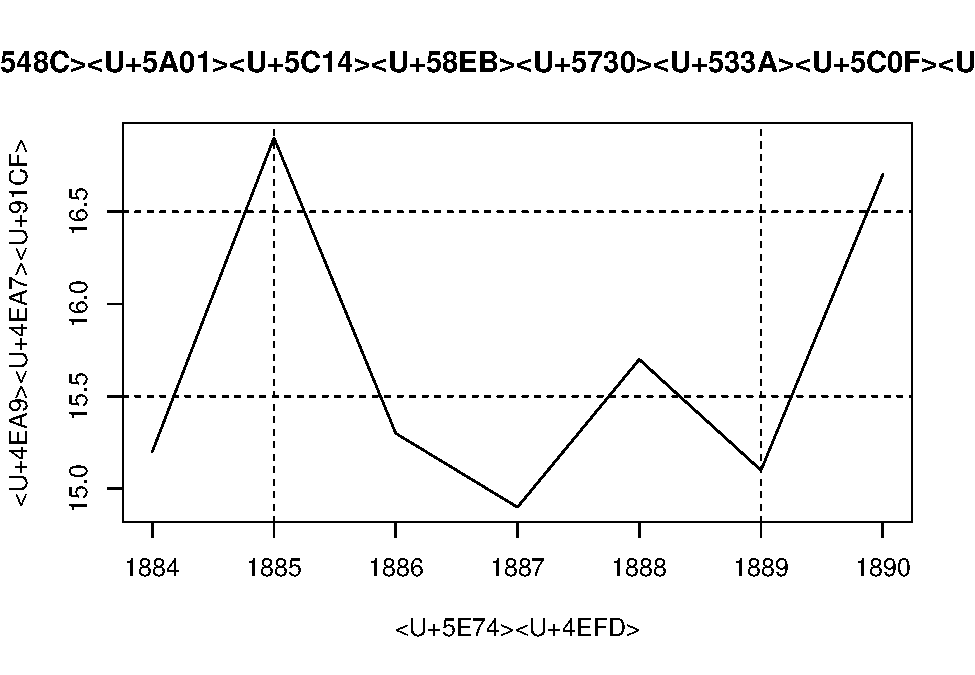
\includegraphics{timeseries_files/figure-latex/unnamed-chunk-7-1.pdf}

\texttt{plot}各项参数:

\begin{Shaded}
\begin{Highlighting}[]
\ControlFlowTok{if}\NormalTok{(}\OtherTok{FALSE}\NormalTok{) \{}
\NormalTok{  type =}\StringTok{ "p"}  \CommentTok{# 点}
         \StringTok{"l"}  \CommentTok{# 线}
         \StringTok{"b"}  \CommentTok{# 点连线}
         \StringTok{"o"}  \CommentTok{# 线穿过点}
         \StringTok{"h"}  \CommentTok{# 悬垂线}
         \StringTok{"s"}  \CommentTok{# 阶梯线}
\NormalTok{  pch =}\StringTok{ }\DecValTok{17} \CommentTok{# 点的符号}
\NormalTok{  lty =}\StringTok{ }\DecValTok{2}  \CommentTok{# 连线的类型}
\NormalTok{  lwd =}\StringTok{ }\DecValTok{2}  \CommentTok{# 连线的宽度(默认宽度的2倍)}
\NormalTok{  col =}\StringTok{ }\DecValTok{1}  \CommentTok{# col = "black"}
\NormalTok{  col =}\StringTok{ }\DecValTok{2}  \CommentTok{# col = "red"}
\NormalTok{  col =}\StringTok{ }\DecValTok{3}  \CommentTok{# col = "green"}
\NormalTok{  col =}\StringTok{ }\DecValTok{4}  \CommentTok{# col = "blue"}
\NormalTok{  xlim =}\StringTok{ }\KeywordTok{c}\NormalTok{(}\DecValTok{1886}\NormalTok{,}\DecValTok{1890}\NormalTok{)}
\NormalTok{  ylim =}\StringTok{ }\KeywordTok{c}\NormalTok{(}\DecValTok{15}\NormalTok{,}\DecValTok{16}\NormalTok{) }\CommentTok{# 指定坐标轴范围}
\NormalTok{\}}
\end{Highlighting}
\end{Shaded}

\hypertarget{ux81eaux76f8ux5173ux56fe}{%
\subparagraph{自相关图}\label{ux81eaux76f8ux5173ux56fe}}

自相关图是一个平面悬垂线图,横坐标表示延迟期数,纵坐标表示自相关系数,悬垂线表示自相关系数的大小。

\begin{Shaded}
\begin{Highlighting}[]
\KeywordTok{acf}\NormalTok{(yield) }\CommentTok{#虚线为自相关系数 2倍标准差位置}
\end{Highlighting}
\end{Shaded}

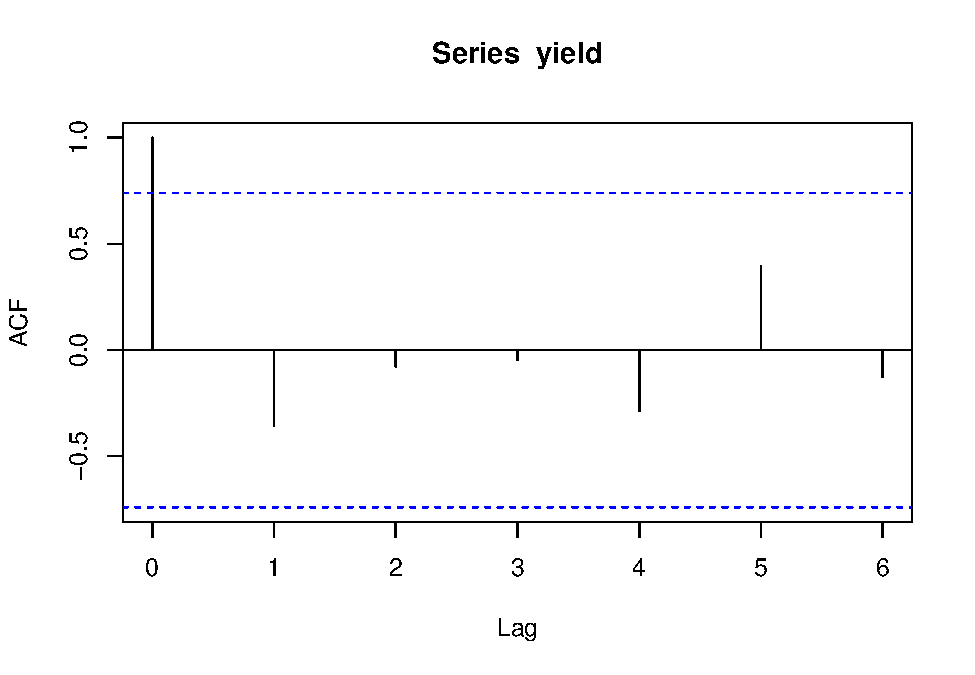
\includegraphics{timeseries_files/figure-latex/unnamed-chunk-9-1.pdf}

\hypertarget{ux5e73ux7a33ux6027ux7684ux68c0ux9a8cux56feux68c0ux9a8cux65b9ux6cd5}{%
\paragraph{平稳性的检验(图检验方法)}\label{ux5e73ux7a33ux6027ux7684ux68c0ux9a8cux56feux68c0ux9a8cux65b9ux6cd5}}

\begin{itemize}
\item
  \textbf{时序图检验}:始终在一个常数值附近随机波动,而且波动的范围有界、无明显趋势及周期特征。
\item
  \textbf{自相关图检验}:平稳序列通常具有短期相关性。该性质用自相关系数来描述就是随着延迟期数的增加,平稳序列的自相关系数会很快地衰减向零。
\end{itemize}

\hypertarget{ux4f8b2.1-ux68c0ux9a8c1964ux5e74-1999ux5e74ux4e2dux56fdux7eb1ux5e74ux4ea7ux91cfux5e8fux5217ux7684ux5e73ux7a33ux6027}{%
\paragraph{例2.1
检验1964年-1999年中国纱年产量序列的平稳性}\label{ux4f8b2.1-ux68c0ux9a8c1964ux5e74-1999ux5e74ux4e2dux56fdux7eb1ux5e74ux4ea7ux91cfux5e8fux5217ux7684ux5e73ux7a33ux6027}}

\begin{Shaded}
\begin{Highlighting}[]
\KeywordTok{library}\NormalTok{(readr)}
\NormalTok{sha <-}\StringTok{ }\KeywordTok{read_csv}\NormalTok{(}\StringTok{"timeseries_data/file4.csv"}\NormalTok{)}
\NormalTok{output <-}\StringTok{ }\KeywordTok{ts}\NormalTok{(sha}\OperatorTok{$}\NormalTok{output, }\DataTypeTok{start =} \DecValTok{1964}\NormalTok{)}
\KeywordTok{plot}\NormalTok{(output, }\DataTypeTok{main =} \StringTok{"时序图"}\NormalTok{)}
\end{Highlighting}
\end{Shaded}

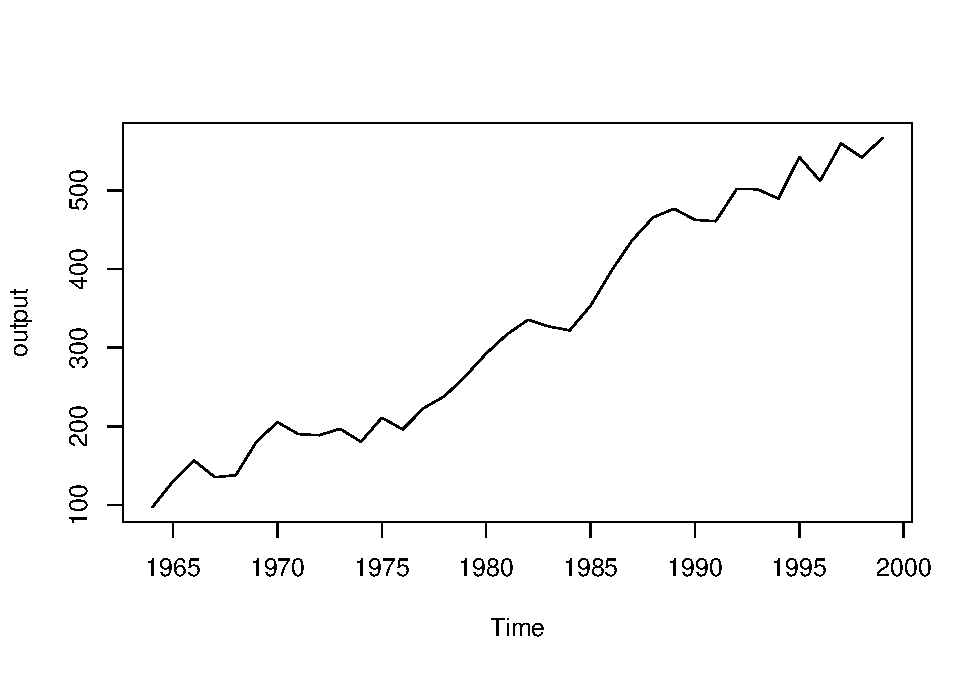
\includegraphics{timeseries_files/figure-latex/ex2.1-1.pdf}

时序图有递增趋势,非平稳

\begin{Shaded}
\begin{Highlighting}[]
\KeywordTok{acf}\NormalTok{(output, }\DataTypeTok{lag =} \DecValTok{25}\NormalTok{,}
    \DataTypeTok{main =} \StringTok{"自相关图"}\NormalTok{)}
\end{Highlighting}
\end{Shaded}

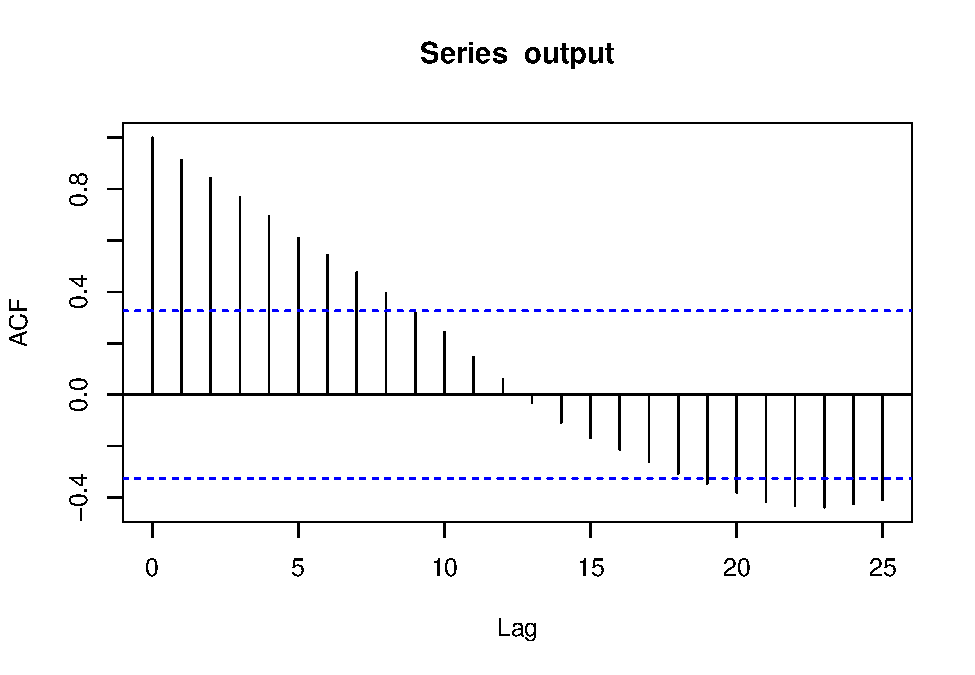
\includegraphics{timeseries_files/figure-latex/2.1acf-1.pdf}

自相关图衰减缓慢,非平稳。


\end{document}
